\documentclass{beamer}
\usetheme{Darmstadt}

\usepackage{color}
\usepackage{listings}
\usepackage{graphicx}
\usepackage{wrapfig}
\usepackage{amsmath}

\setbeamertemplate{frametitle}[default][center]
\beamertemplatenavigationsymbolsempty

\title{Utilizing Crowd Intelligence for Online Detection of Emotional Distress}
\subtitle{Master's Thesis Presentation}
\author[Siddhant Goel]{Siddhant Goel\\{\small Advisor: Han Xiao\\Supervisor: Prof. Dr. Claudia Eckert}}
\institute{
Chair for IT Security\\
Technische Universit\"at M\"unchen
}
\date{\today}

\begin{document}
    \begin{frame}[plain]
        \titlepage
    \end{frame}
    
    \begin{frame}
        \frametitle{Outline}
        \begin{itemize}
            \item{
            Introduction
            \begin{itemize}
                \item{Backdrop}
                \item{Motivation}
                \item{Problem Definition}
            \end{itemize}
            }
            \item{
            Theoretical Background
            \begin{itemize}
                \item{Machine Learning and Text Classification}
                \item{Support Vector Machines}
                \item{Ensemble Learning methods}
            \end{itemize}
            }
            \item{
            Experimental Results
            \begin{itemize}
                \item{Experiments}
                \item{Results}
            \end{itemize}
            }
            \item{Conclusion and Future Work}
            \item{Q/A}
        \end{itemize}
    \end{frame}
    
    \begin{frame}
        \begin{center}
            \textbf{Introduction}
        \end{center}
    \end{frame}
    
    \begin{frame}
        \frametitle{Backdrop}
        \begin{itemize}
            \item{Millions of people die every year because of suicide}
            \item{Most people are between 15 to 29 years old}
            \item{Rise of social media - Twitter, Facebook, Reddit, Wordpress}
            \item{Sections of interest on Reddit - ``/r/happy'' \footnote{\url{http://www.reddit.com/r/happy}} and ``/r/suicidewatch'' \footnote{\url{http://www.reddit.com/r/suicidewatch}}}
            \item{Sections of interest on Twitter - the entire website}
            \item{People want to post their inner feelings on the web}
            \item{\textbf{Direct phrases} - \emph{``thoughts of suicide make me happy''}, \emph{``I have a rope around my neck''}}
            \item{\textbf{Indirect phrases} - \emph{``I don't know anything anymore''}, \emph{``Need someone to talk to''}}
        \end{itemize}
    \end{frame}
    
    \begin{frame}
        \frametitle{Backdrop}
        \begin{figure}
            \centering
            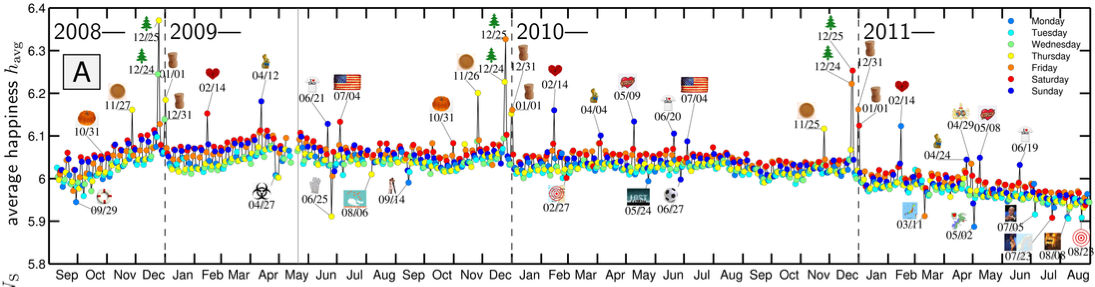
\includegraphics[width=\textwidth]{figures/twitter_happiness.png}
            \caption{Happiness on Twitter as a function of time}
        \end{figure}
        \begin{itemize}
            \item{Study conducted in 2011}
            \item{46 billion words collected over 33 months}
            \item{Negativity on Twitter has been on the rise}
            \item{Words include \emph{death}, \emph{hate}, and even \emph{suicide}}
        \end{itemize}
    \end{frame}
    
    \begin{frame}
        \frametitle{Motivation}
        \begin{figure}
            \centering
            
\includegraphics[width=0.5\textwidth]{figures/twitter_kcs.png}
            \caption{Last tweet of Twitter user ``@CapitalSTEEZ\_''\footnote{\url{http://twitter.com/CapitalSteez\_}}}
        \end{figure}
        \begin{itemize}
            \item{Some accounts have lots of followers, some don't}
            \item{Lives can be saved if there is a surveillance system of suicide}
            \item{Public sentiment information available on the web + No analysis possible = Disconnect}
        \end{itemize}
    \end{frame}
    
    \begin{frame}
        \frametitle{Problem Definition}
        \begin{itemize}
            \item{Evaluate machine learning algorithms that can be used for identifying depressed emotions in pieces of text}
            \item{
            Build a web based system that can
            \begin{itemize}
                \item{tap into crowd intelligence to incrementally improve the classifiers}
                \item{detect content on the web that indicates that its author may be depressed or suicidal}
            \end{itemize}
            }
        \end{itemize}
    \end{frame}
    
    \begin{frame}
        \begin{center}
            \textbf{Theoretical Background}
        \end{center}
    \end{frame}
    
    \begin{frame}
        \frametitle{Machine Learning}
        \begin{itemize}
            \item{Algorithms that can learn from data}
            \item{Construct a model from a given dataset, and then perform the required task on another dataset}
            \item{\textbf{Supervised learning} - Train the models on the training data, and predict on the test data}
            \item{\textbf{Unsupervised learning} - No distinction between training and test data}
        \end{itemize}
    \end{frame}
    
    \begin{frame}
        \frametitle{Text Classification}
        \begin{itemize}
            \item{Subset of machine learning algorithms (we focus on supervised text classification)}
            \item{Given some pieces of text, put unseen pieces of text into two or more categories}
            \item{Dataset $\{(\mathbf{x_n}, y_n)\}_{n = 1}^{N}$ containing N instances}
            \item{Each instance $(\mathbf{x_n}, y_n)$ is of the form $[(x_{n, 1}, x_{n, 2}, ..., x_{n, D}), y_n]$}
            \item{Supervised learning - calculate $y_n$ of test data given information about $y_n$ from training data}
            \item{Unsupervised learning - calculate $y_n$ given only information about $\mathbf{x_n}$}
        \end{itemize}
    \end{frame}
    
    \begin{frame}
        \frametitle{Support Vector Machines}
        \begin{itemize}
            \item{Fairly popular class of algorithms used for binary classification}
            \item{Given training data in some $D$ dimensional space, find a decision boundary (hyperplane) that separates the two classes}
            \item{Maximize the distance of the boundary from any data point}
            \item{Decision function depends on a (usually small) subset of points called support vectors}
            \item{Kernel (linear/polynomial/RBF/Sigmoid) functions used to calculate distance between two points}
        \end{itemize}
    \end{frame}
    
    \begin{frame}
        \frametitle{Linear kernel SVM}
        \begin{figure}
            \centering
            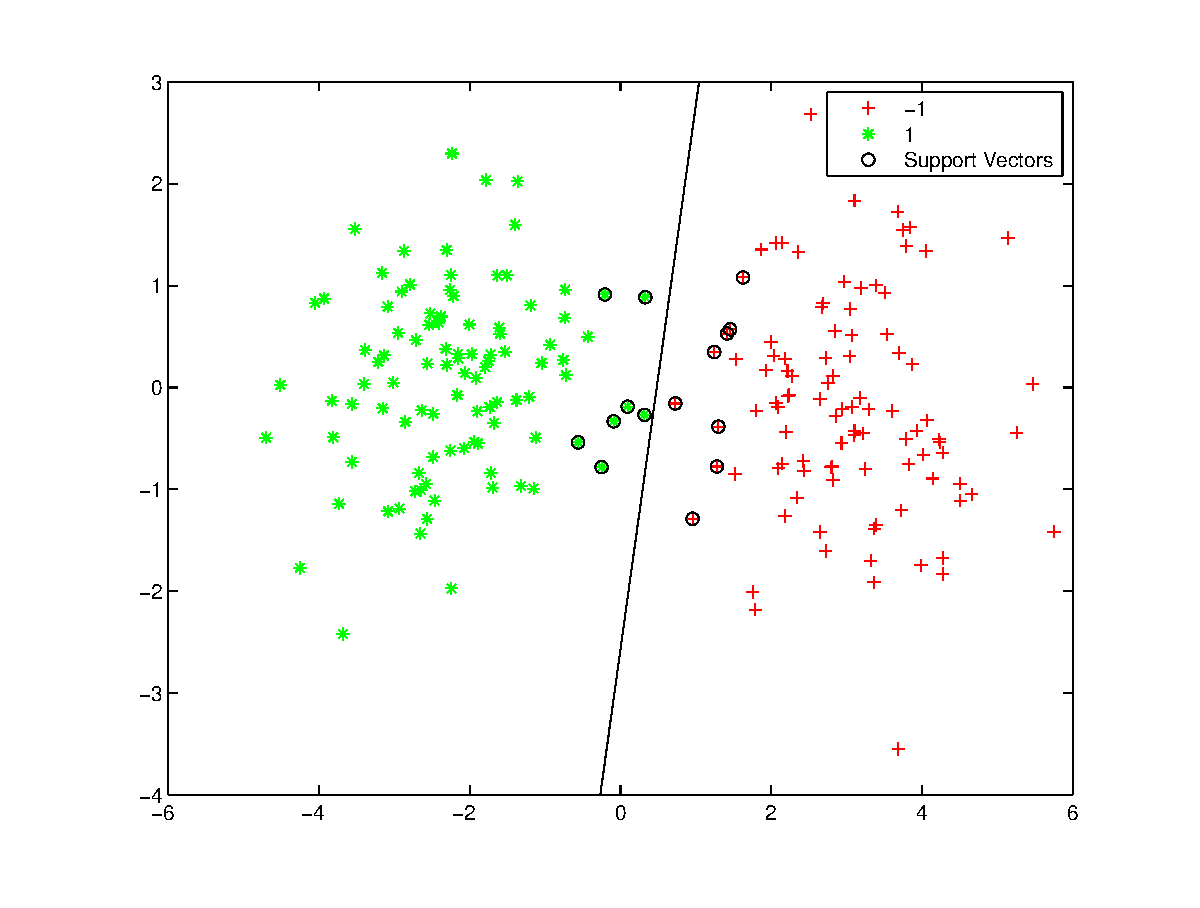
\includegraphics[width=0.5\textwidth]{figures/svm_linear_classification.eps}
            \caption{Binary classification on a dataset using a linear kernel SVM}
        \end{figure}
    \end{frame}
    
    \begin{frame}
        \frametitle{Kernel functions}
        \begin{columns}
            \begin{column}{0.4\textwidth}
                \begin{figure}
                    \centering
                    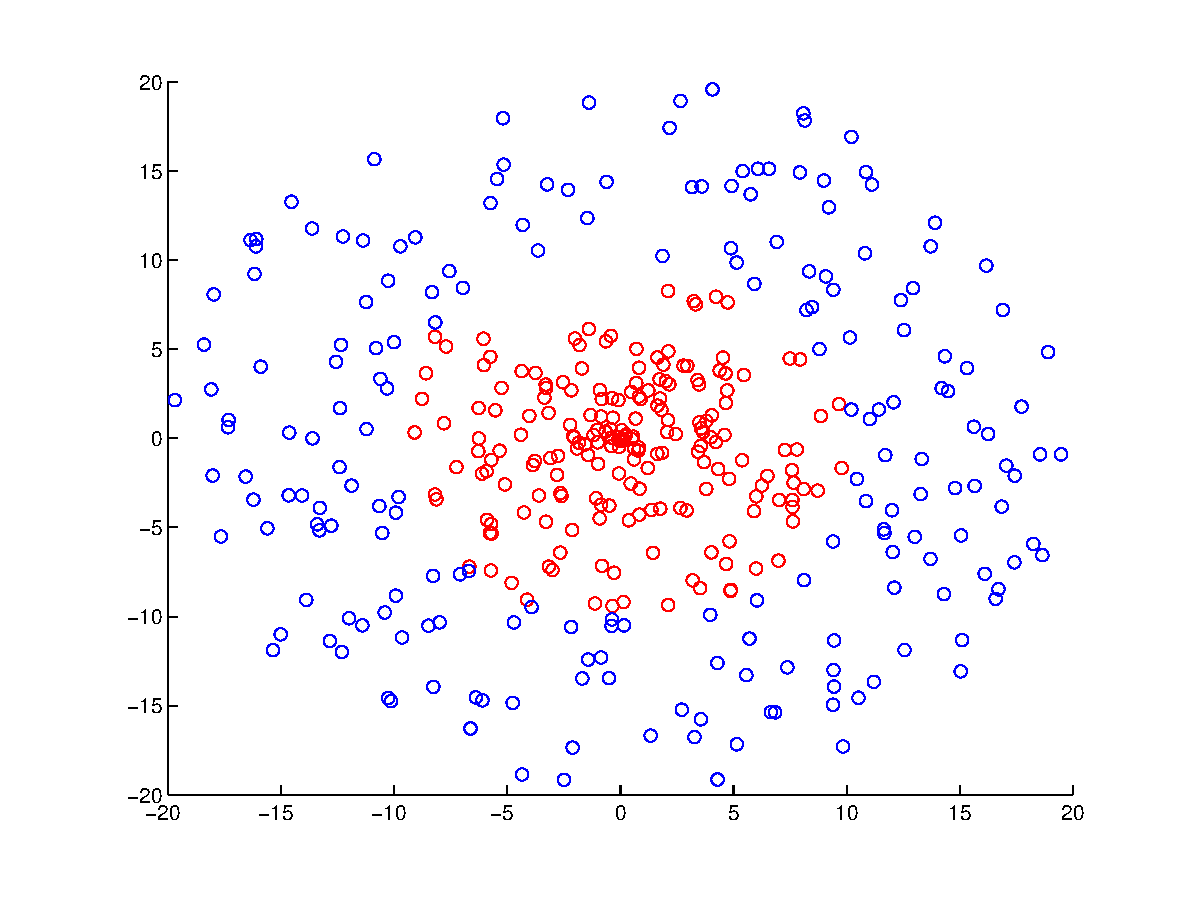
\includegraphics[width=\textwidth]{figures/svm_non_linear_data.eps}
                    \caption{Dataset in 2D (cannot be classified using a linear kernel SVM)}
                \end{figure}
            \end{column}
            \begin{column}{0.2\textwidth}
                \begin{center}
                    $\xrightarrow{x_3 = \sqrt{x_1^2 + x_2^2}}$
                \end{center}
            \end{column}
            \begin{column}{0.4\textwidth}
                \begin{figure}
                    \centering
                    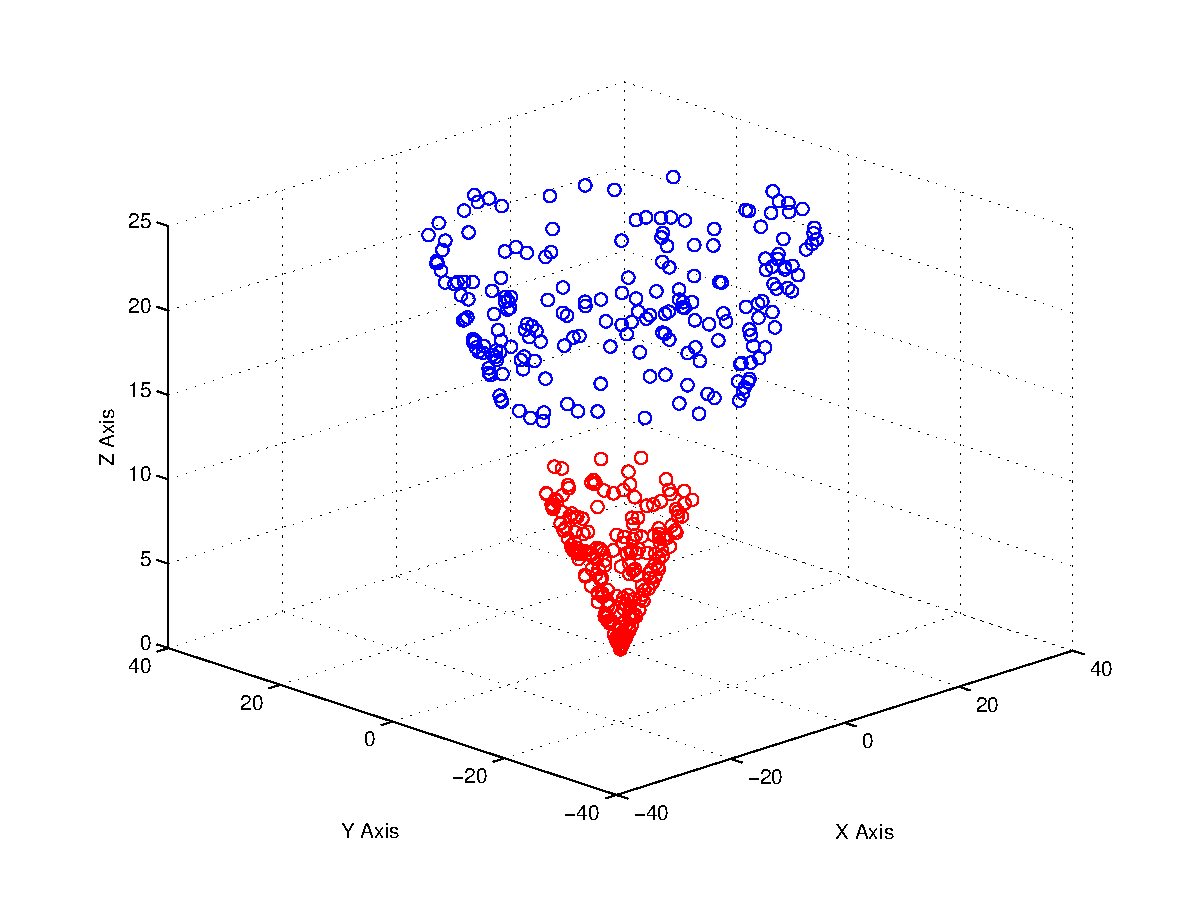
\includegraphics[width=\textwidth]{figures/svm_non_linear_data_3d.eps}
                    \caption{Dataset transformed to 3D}
                \end{figure}
            \end{column}
        \end{columns}
    \end{frame}
    
    \begin{frame}
        \frametitle{Ensemble Learning}
        \begin{itemize}
            \item{Class of machine learning methods that combine models to obtain better predictions}
            \item{Performance not guaranteed to be better than constituent classifiers}
            \item{Ensemble methods still usually outperform individual classifiers}
            \item{Soft requirement - underlying models should be diverse}
            \item{Various strategies to combine models - \emph{select best}, \emph{voting}, \emph{boosting}, \emph{stacking}}
        \end{itemize}
    \end{frame}
    
    \begin{frame}
        \frametitle{Bagging}
        \begin{itemize}
            \item{Combine $M$ classifiers to form a single classifier}
            \item{To predict, obtain predictions from all constituent classifiers, and take majority vote}
            \item{Requirement - classifiers should change for even small changes in underlying classifiers}
            \item{
            Two main approaches for training individual classifiers
            \begin{itemize}
                \item{Sample split - different samples for different classifiers}
                \item{Feature split - different features for different classifiers}
            \end{itemize}
            }
        \end{itemize}
    \end{frame}
    
    \begin{frame}
        \frametitle{Boosting}
        \begin{itemize}
            \item{Assign each sample a weight value (same for all samples in the beginning)}
            \item{Train $M$ classifiers successively}
            \item{Each classifier focuses more on samples that the previous classifier classified incorrectly}
            \item{For each classifier, calculate $\epsilon$ (measure of error) and $\alpha$ (decreases with $\epsilon$)}
            \item{Final prediction = $\mathrm{sign}(\displaystyle \sum_{m = 1}^{M} \alpha_m y_m(\mathbf{x_n}))$}
        \end{itemize}
    \end{frame}
    
    \begin{frame}
        \frametitle{Stacking}
        \begin{figure}
            \centering
            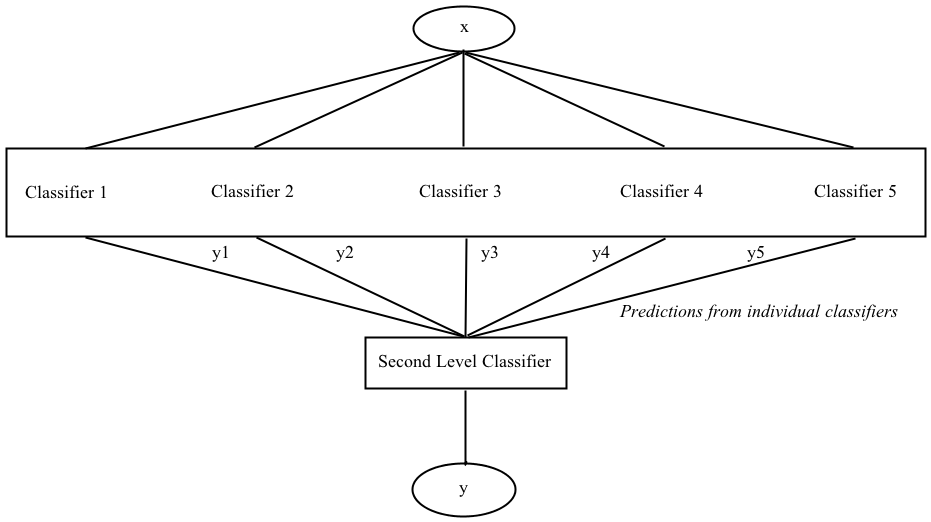
\includegraphics[width=0.7\textwidth]{figures/stacking_prediction_flow.png}
            \caption{Prediction using a stacking ensemble}
        \end{figure}
        \begin{itemize}
            \item{Outputs from first layer form the input for second layer}
            \item{Layer-1 classifiers can be trained using bootstrapping or selecting random features}
        \end{itemize}
    \end{frame}
    
    \begin{frame}
        \begin{center}
            \textbf{Experimental Results}
        \end{center}
    \end{frame}
    
    \begin{frame}
        \begin{center}
            \textbf{Experiments}
        \end{center}
    \end{frame}
    
    \begin{frame}
        \frametitle{Evaluation of algorithms}
        \begin{center}
            \textbf{Approach}
        \end{center}
        \begin{itemize}
            \item{Implement all the models in MATLAB}
            \item{Extract n-grams (size upto 2) out of the Kaggle dataset}
            \item{Use tf-idf information as feature values}
            \item{Input matrix - 6182 rows and 23175 columns}
            \item{\textbf{SVM}, \textbf{Bagging}, \textbf{Boosting}, \textbf{Stacking} - obtain accuracy (10-fold cross validation) against number of samples}
            \item{\textbf{SVM} - Growth of number of support vectors with the number of samples}
            \item{\textbf{Bagging} - Accuracy against number of underlying models}
            \item{Start with 100 samples, and continue adding 100 samples on each iteration until no more samples are left}
        \end{itemize}
    \end{frame}
    
    \begin{frame}
        \begin{center}
            \textbf{Results}
        \end{center}
    \end{frame}
    
    \begin{frame}
        \frametitle{Evaluation of algorithms}
        \begin{center}
            \textbf{Support Vector Machines}
        \end{center}
        \begin{columns}
            \begin{column}{0.5\textwidth}
                \begin{figure}
                    \centering
                    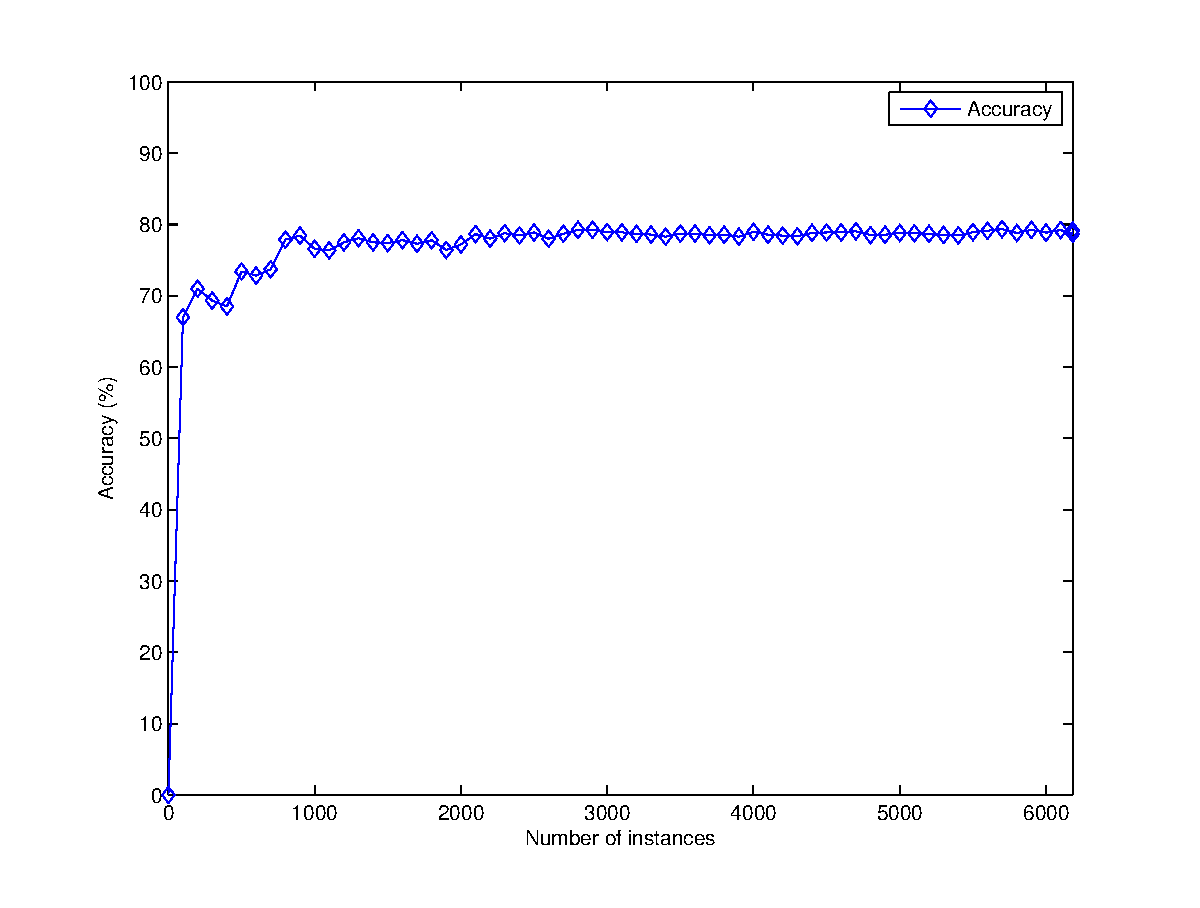
\includegraphics[width=\textwidth]{figures/svm_accuracy.eps}
                    \caption{Accuracy v/s Number of instances}
                \end{figure}
            \end{column}
            \begin{column}{0.5\textwidth}
                \begin{itemize}
                    \item{Linear kernel accuracy - 79.02\%}
                    \item{Polynomial/RBF/Sigmoid kernel accuracy - 34.39\%}
                    \item{Having more features implies no need for a kernel function}
                \end{itemize}
            \end{column}
        \end{columns}
    \end{frame}
    
    \begin{frame}
        \frametitle{Evaluation of algorithms}
        \begin{center}
            \textbf{Support Vector Machines}
        \end{center}
        \begin{columns}
            \begin{column}{0.5\textwidth}
                \begin{figure}
                    \centering
                    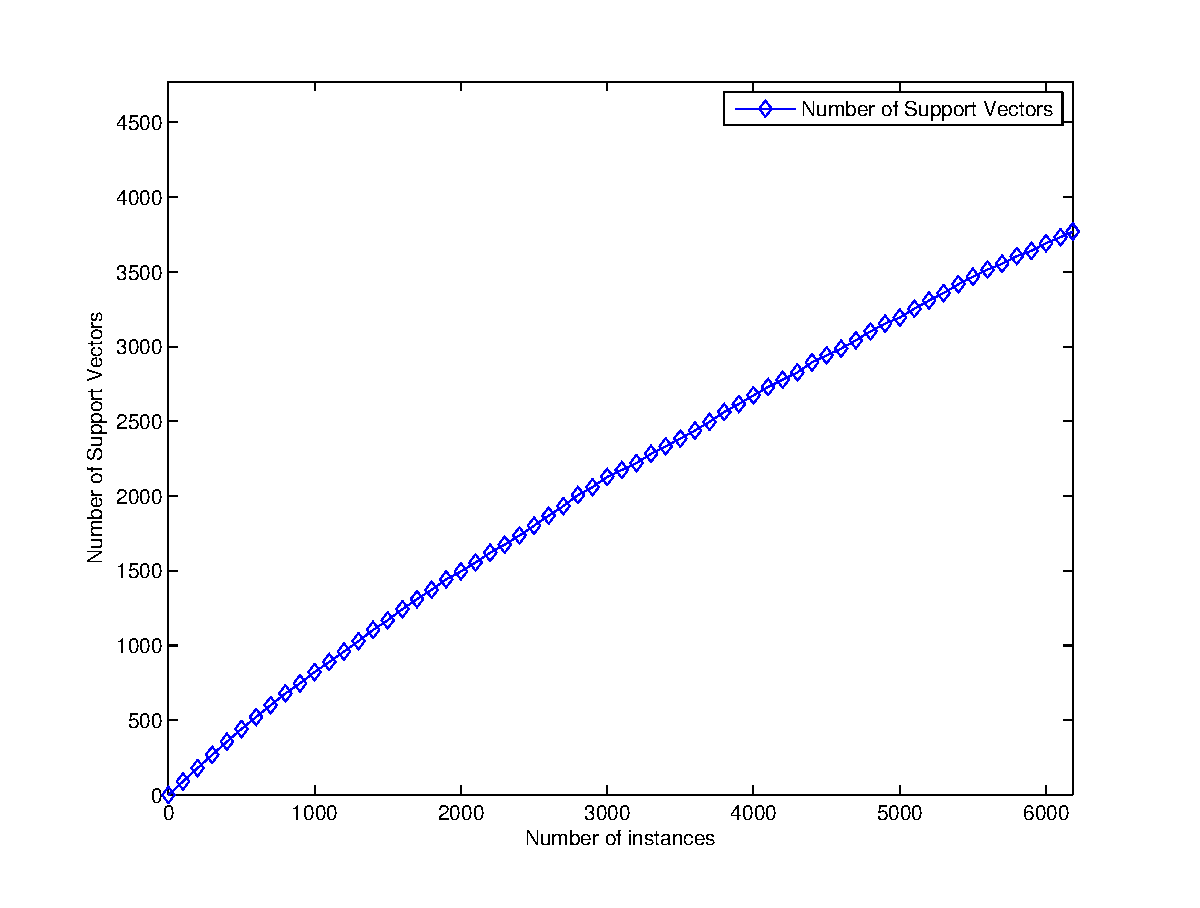
\includegraphics[width=\textwidth]{figures/svm_n_sv.eps}
                    \caption{Number of support vectors v/s Number of instances}
                \end{figure}
            \end{column}
            \begin{column}{0.5\textwidth}
                \begin{itemize}
                    \item{100 samples - 90\% support vectors}
                    \item{6182 samples - 60\% support vectors}
                    \item{Less support vectors implies that the classification is easy}
                \end{itemize}
            \end{column}
        \end{columns}
    \end{frame}
    
    \begin{frame}
        \frametitle{Evaluation of algorithms}
        \begin{center}
            \textbf{Bagging}
        \end{center}
        \begin{columns}
            \begin{column}{0.5\textwidth}
                \begin{figure}
                    \centering
                    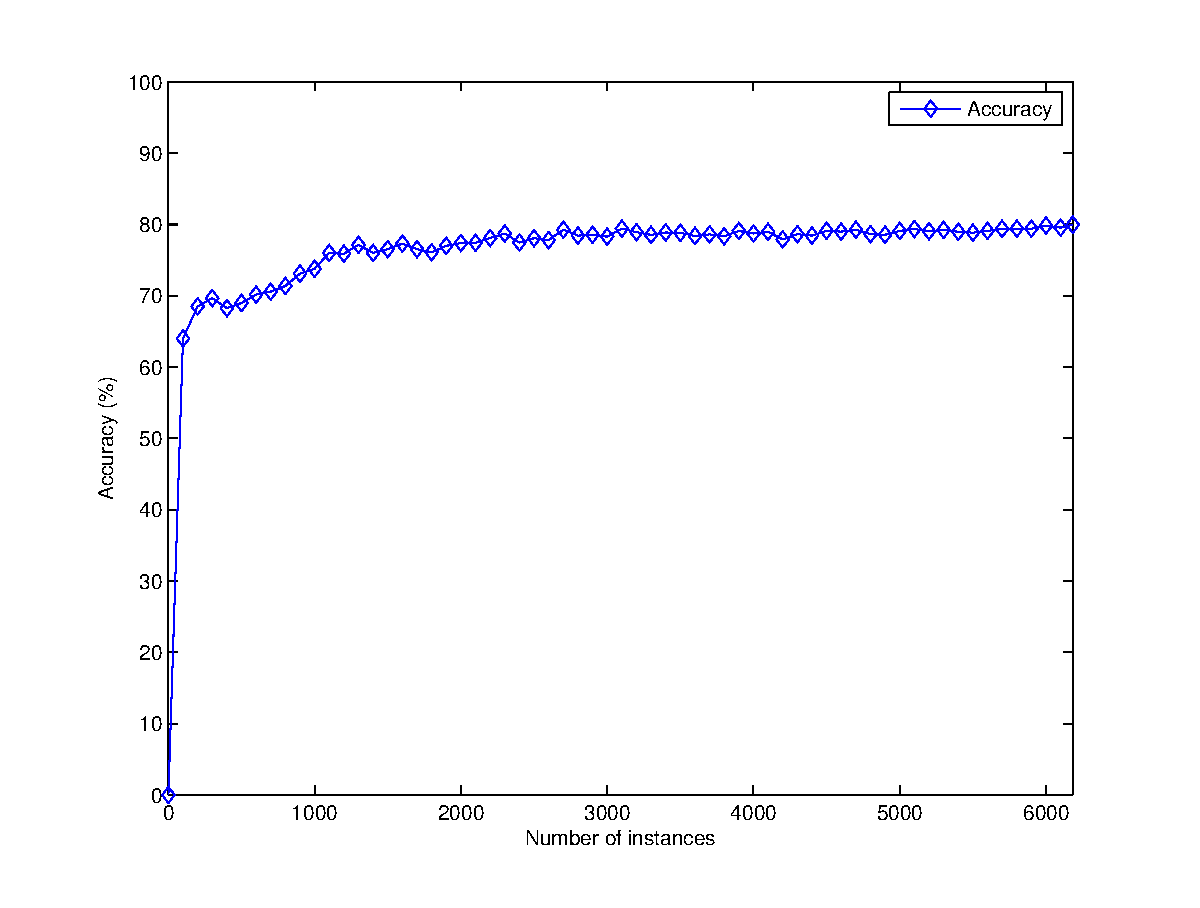
\includegraphics[width=\textwidth]{figures/bagging_accuracy.eps}
                    \caption{Accuracy v/s Number of instances}
                \end{figure}
            \end{column}
            \begin{column}{0.5\textwidth}
                \begin{itemize}
                    \item{9 linear kernel SVMs underneath}
                    \item{Performance ultimately governed by how SVMs perform}
                    \item{Average accuracy on all 6182 samples = 79.65\%}
                \end{itemize}
            \end{column}
        \end{columns}
    \end{frame}
    
    \begin{frame}
        \frametitle{Evaluation of algorithms}
        \begin{center}
            \textbf{Bagging}
        \end{center}
        \begin{columns}
            \begin{column}{0.5\textwidth}
                \begin{figure}
                    \centering
                    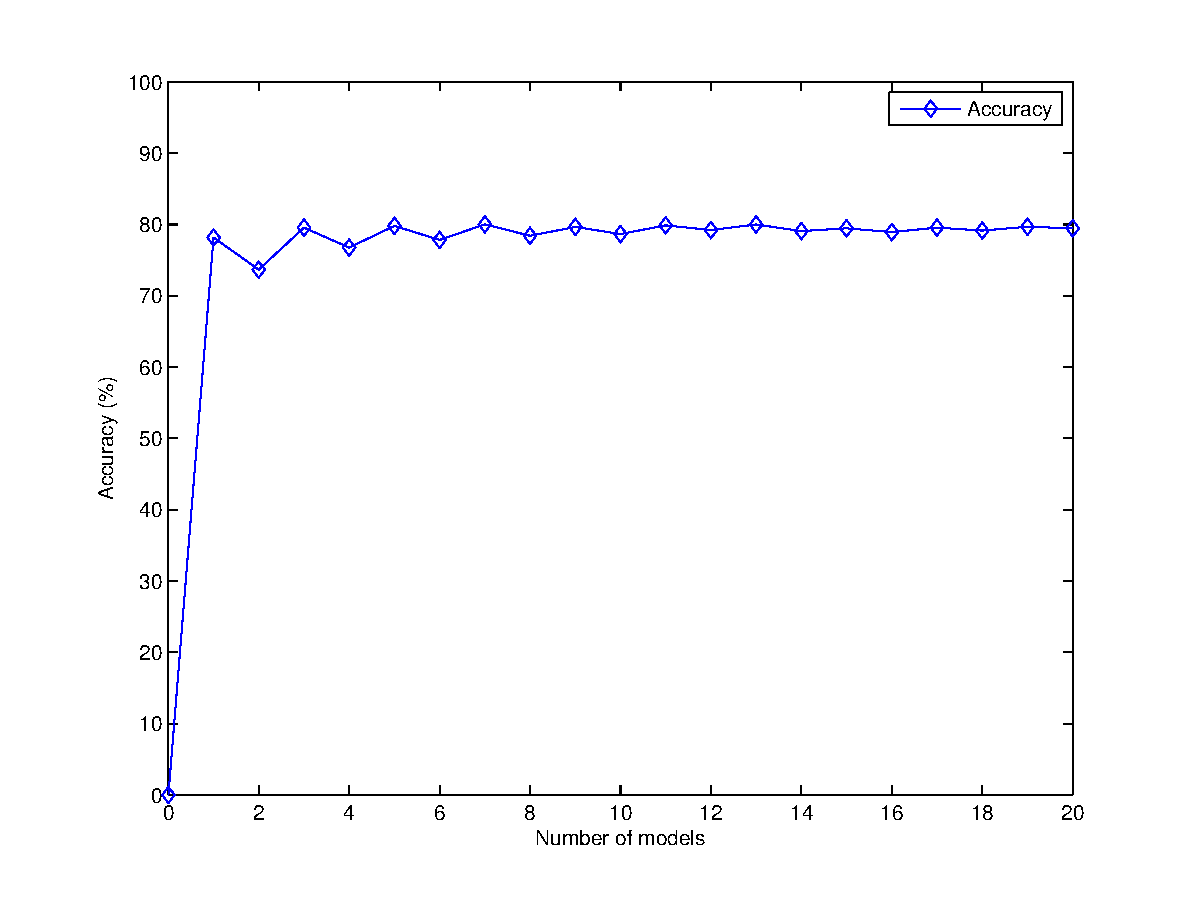
\includegraphics[width=\textwidth]{figures/bagging_n_models.eps}
                    \caption{Accuracy v/s Number of models}
                \end{figure}
            \end{column}
            \begin{column}{0.5\textwidth}
                \begin{itemize}
                    \item{Accuracy ``stabilizes'' slowly with the number of models}
                    \item{Each model is assigned a random subset of samples}
                    \item{Increase in number of models \emph{implies} Subsets overlap \emph{implies} Performance stabilizes}
                \end{itemize}
            \end{column}
        \end{columns}
    \end{frame}
    
    \begin{frame}
        \frametitle{Evaluation of algorithms}
        \begin{center}
            \textbf{Boosting}
        \end{center}
        \begin{columns}
            \begin{column}{0.5\textwidth}
                \begin{figure}
                    \centering
                    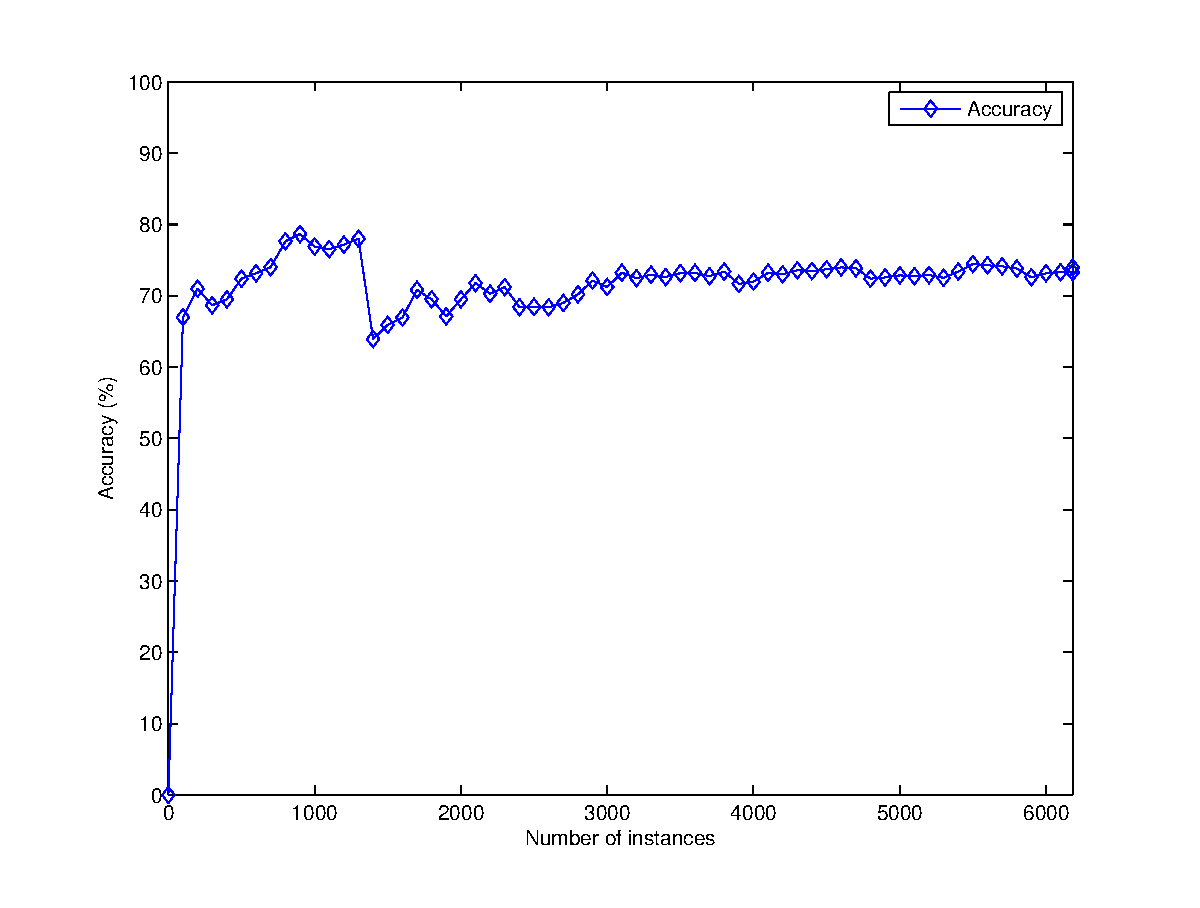
\includegraphics[width=\textwidth]{figures/boosting_accuracy.eps}
                    \caption{Accuracy v/s Number of instances}
                \end{figure}
            \end{column}
            \begin{column}{0.5\textwidth}
                \begin{itemize}
                    \item{9 linear kernel SVMs trained successively on each iteration}
                    \item{Average accuracy = 72.84\%}
                \end{itemize}
            \end{column}
        \end{columns}
    \end{frame}
    
    \begin{frame}
        \frametitle{Evaluation of algorithms}
        \begin{center}
            \textbf{Stacking}
        \end{center}
        \begin{columns}
            \begin{column}{0.5\textwidth}
                \begin{figure}
                    \centering
                    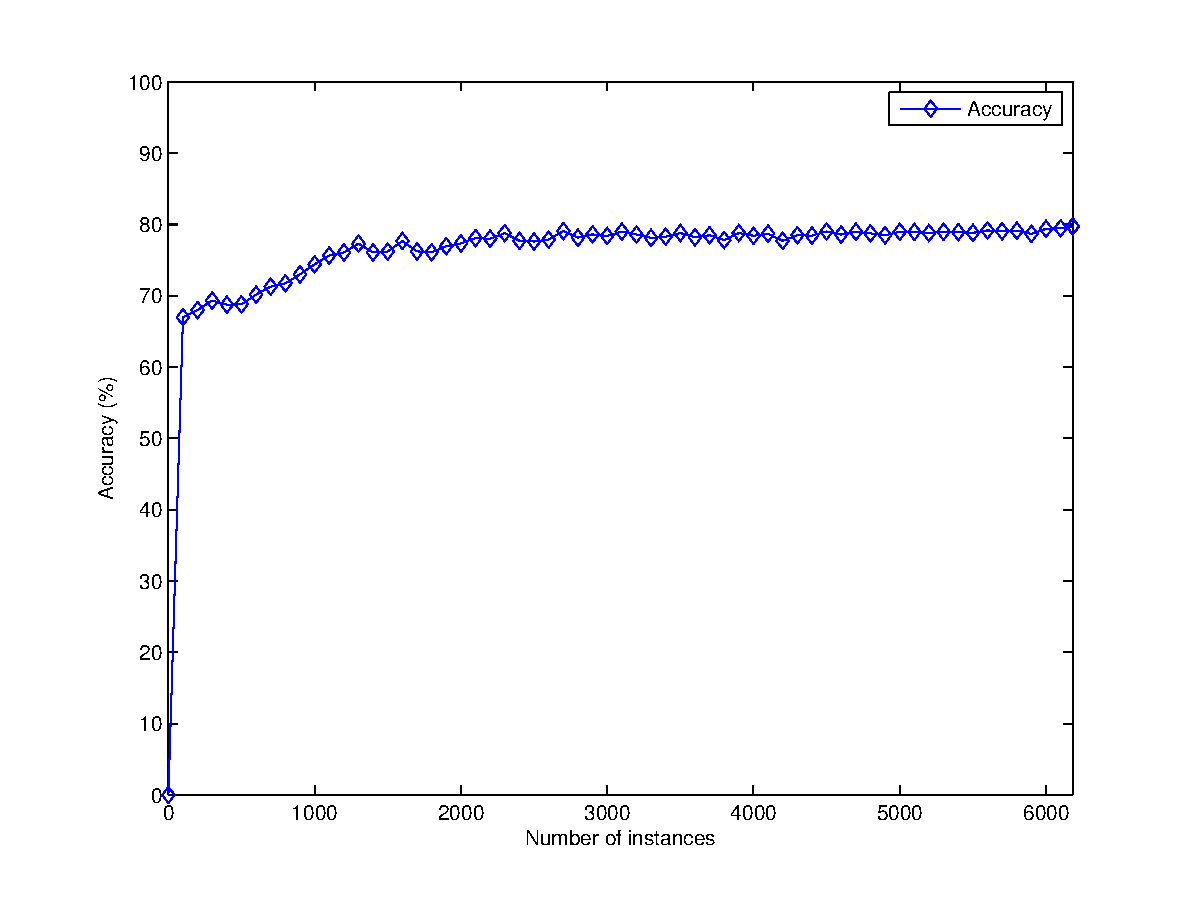
\includegraphics[width=\textwidth]{figures/stacking_accuracy.eps}
                    \caption{Accuracy v/s Number of instances}
                \end{figure}
            \end{column}
            \begin{column}{0.5\textwidth}
                \begin{itemize}
                    \item{9 linear kernel SVMs at first level}
                    \item{Average accuracy = 79.48\%}
                \end{itemize}
            \end{column}
        \end{columns}
    \end{frame}
    
    \begin{frame}
        \frametitle{Web based system}
        \begin{center}
            \textbf{Approach}
        \end{center}
        \begin{itemize}
            \item{Implement all the models in Python, and web interface in Django}
            \item{No training data available $=>$ build our own}
            \item{
            Training data
            \begin{itemize}
                \item{comes from Reddit}
                \item{``/r/happy'' - users posts their happy moments}
                \item{``/r/suicidewatch'' - users post when they want to commit suicide}
                \item{pull 500 stories from each, every day}
            \end{itemize}
            }
            \item{
            Prediction data
            \begin{itemize}
                \item{should be the general sentiment of the overall public}
                \item{hence, Twitter}
                \item{pull 100 tweets every 3 hours}
            \end{itemize}
            }
        \end{itemize}
    \end{frame}
    
    \begin{frame}
        \frametitle{Web based system}
        \begin{center}
            \textbf{Data consolidation frequencies}
        \end{center}
        \begin{table}
            \begin{center}
                \begin{tabular}{ | c | c | }
                    \hline
                    \textbf{Task} & \textbf{Frequency} \\
                    \hline
                    Fetch 1000 posts from Reddit & 24 hours \\
                    \hline
                    Fetch 100 tweets from Twitter & 3 hours \\
                    \hline
                    Re-assign labels to previous tweets and update statistics & 24 hours \\
                    \hline
                \end{tabular}
            \end{center}
        \end{table}
    \end{frame}
    
    \begin{frame}
        \frametitle{Web based system}
        \begin{center}
            \textbf{Architecture}
        \end{center}
        \begin{columns}
            \begin{column}{0.5\textwidth}
                \begin{figure}
                    \centering
                    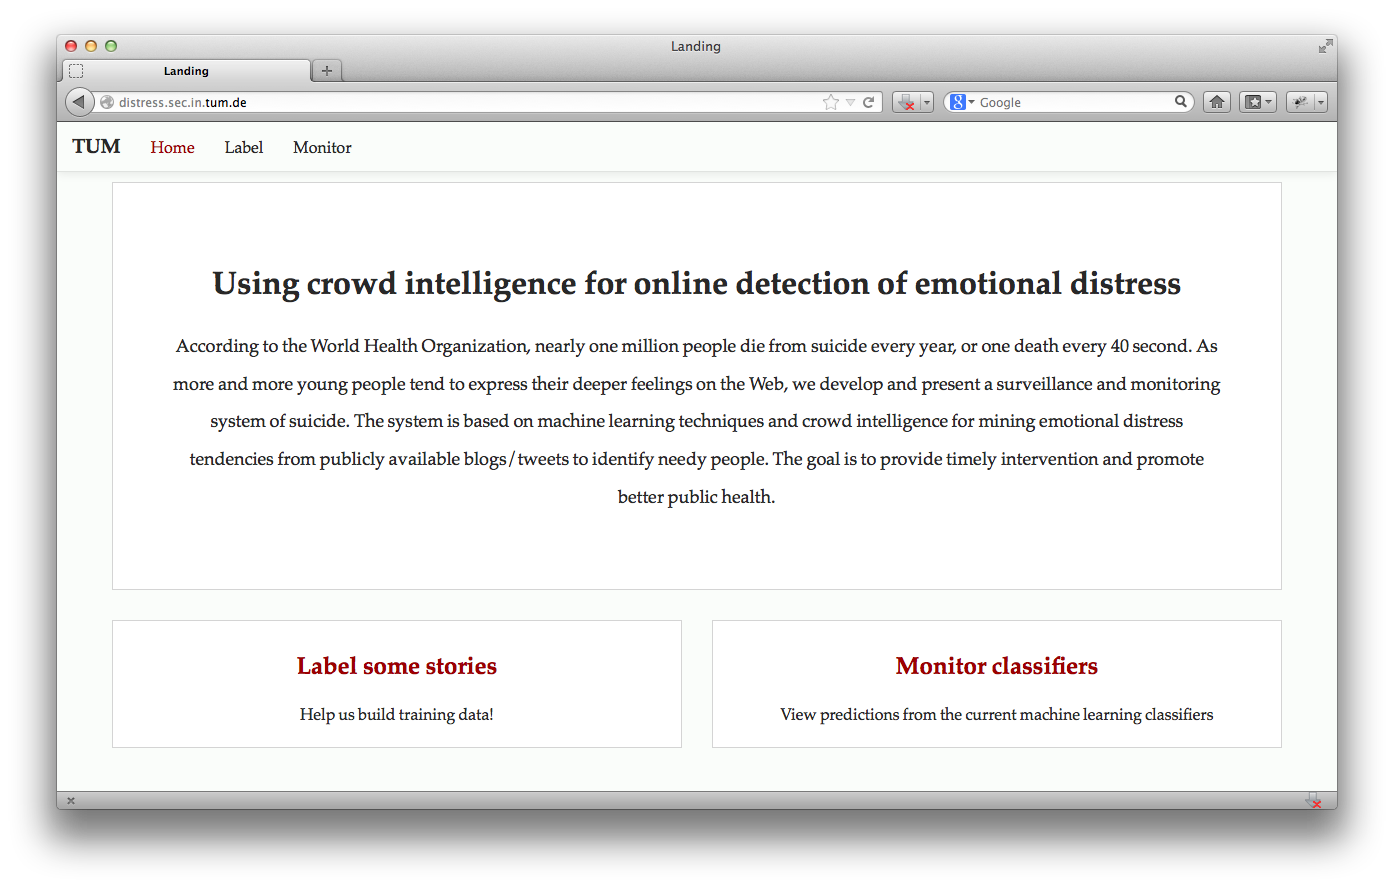
\includegraphics[width=\textwidth]{figures/landing.png}
                    \caption{Landing page}
                \end{figure}
            \end{column}
            \begin{column}{0.5\textwidth}
                \begin{itemize}
                    \item{two sections - \emph{Ratings} and \emph{Monitoring}}
                    \item{\emph{Ratings} - used to build the training data}
                    \item{\emph{Monitoring} - used to monitor the status of the models and check distressed tweets}
                \end{itemize}
            \end{column}
        \end{columns}
    \end{frame}
    
    \begin{frame}
        \frametitle{Web based system}
        \begin{center}
            \textbf{Ratings module}
        \end{center}
        \begin{columns}
            \begin{column}{0.5\textwidth}
                \begin{figure}
                    \centering
                    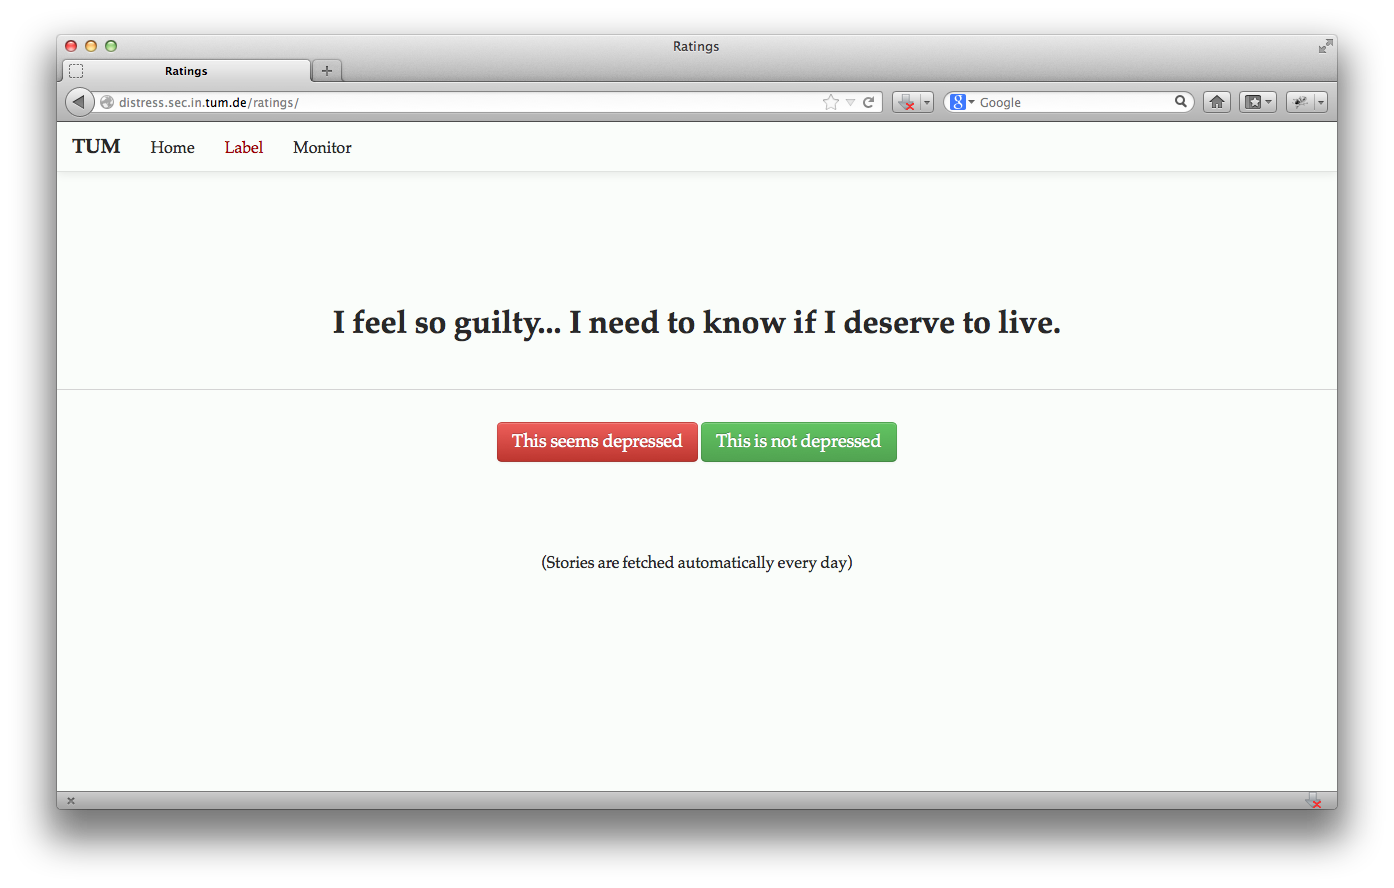
\includegraphics[width=\textwidth]{figures/ratings.png}
                    \caption{Landing page of the Ratings module}
                \end{figure}
            \end{column}
            \begin{column}{0.5\textwidth}
                \begin{itemize}
                    \item{taps into crowd intelligence}
                    \item{automated scripts fetch 1000 posts from Reddit every day}
                    \item{displays the first unlabelled post}
                    \item{users can then assign labels to stories}
                    \item{this builds the training data}
                \end{itemize}
            \end{column}
        \end{columns}
    \end{frame}
    
    \begin{frame}
        \frametitle{Web based system}
        \begin{center}
            \textbf{Monitoring module}
        \end{center}
        \begin{columns}
            \begin{column}{0.5\textwidth}
                \begin{figure}
                    \centering
                    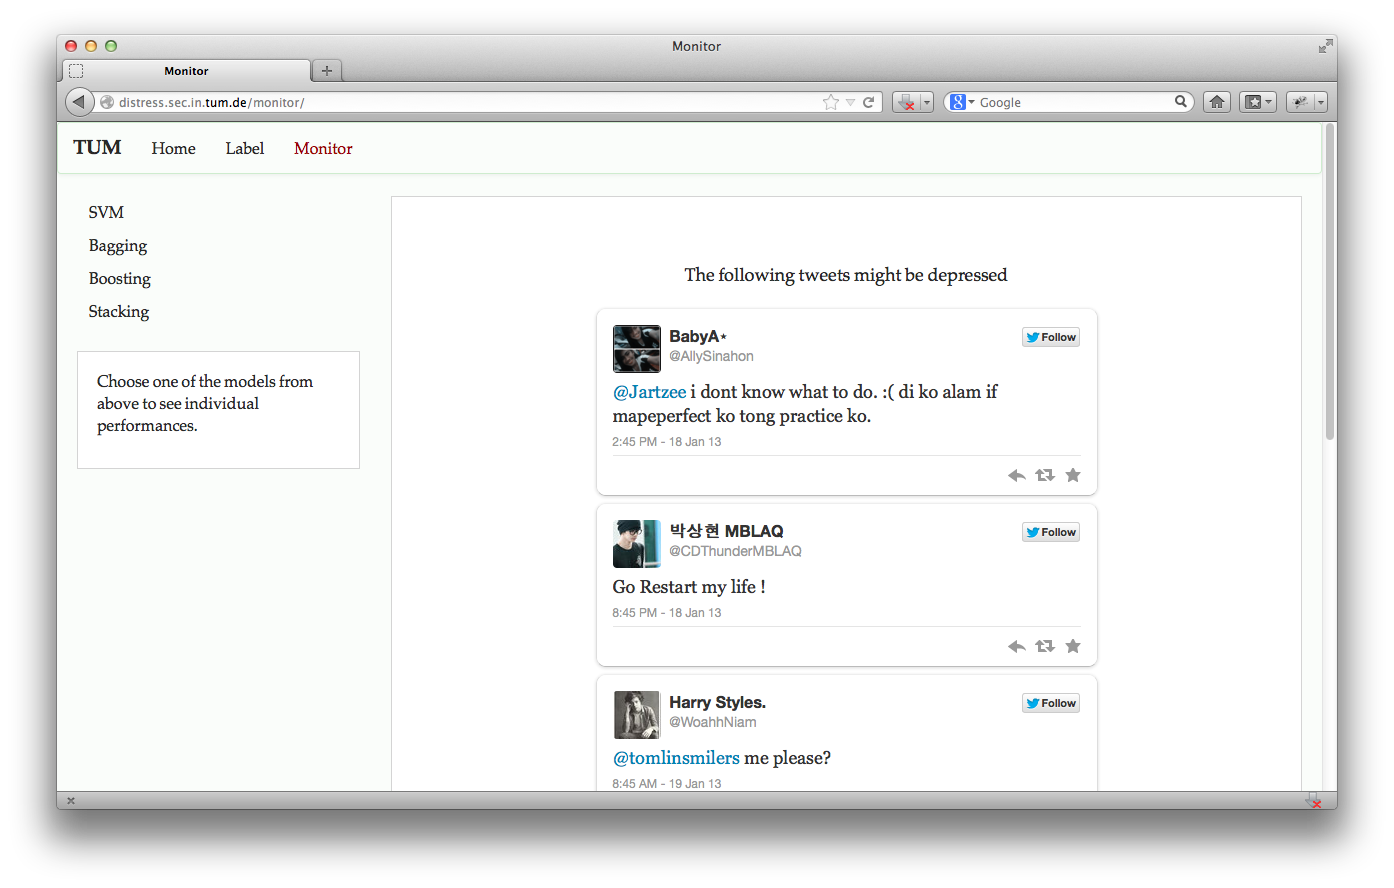
\includegraphics[width=\textwidth]{figures/monitoring_landing_1.png}
                    \caption{Landing page of the Monitoring module}
                \end{figure}
            \end{column}
            \begin{column}{0.5\textwidth}
                \begin{itemize}
                    \item{displays the top few tweets that were classified as depressed by all the classifiers}
                    \item{links for checking the status of individual classifiers}
                \end{itemize}
            \end{column}
        \end{columns}
    \end{frame}
    
    \begin{frame}
        \frametitle{Web based system}
        \begin{center}
            \textbf{Monitoring module}
        \end{center}
        \begin{columns}
            \begin{column}{0.5\textwidth}
                \begin{figure}
                    \centering
                    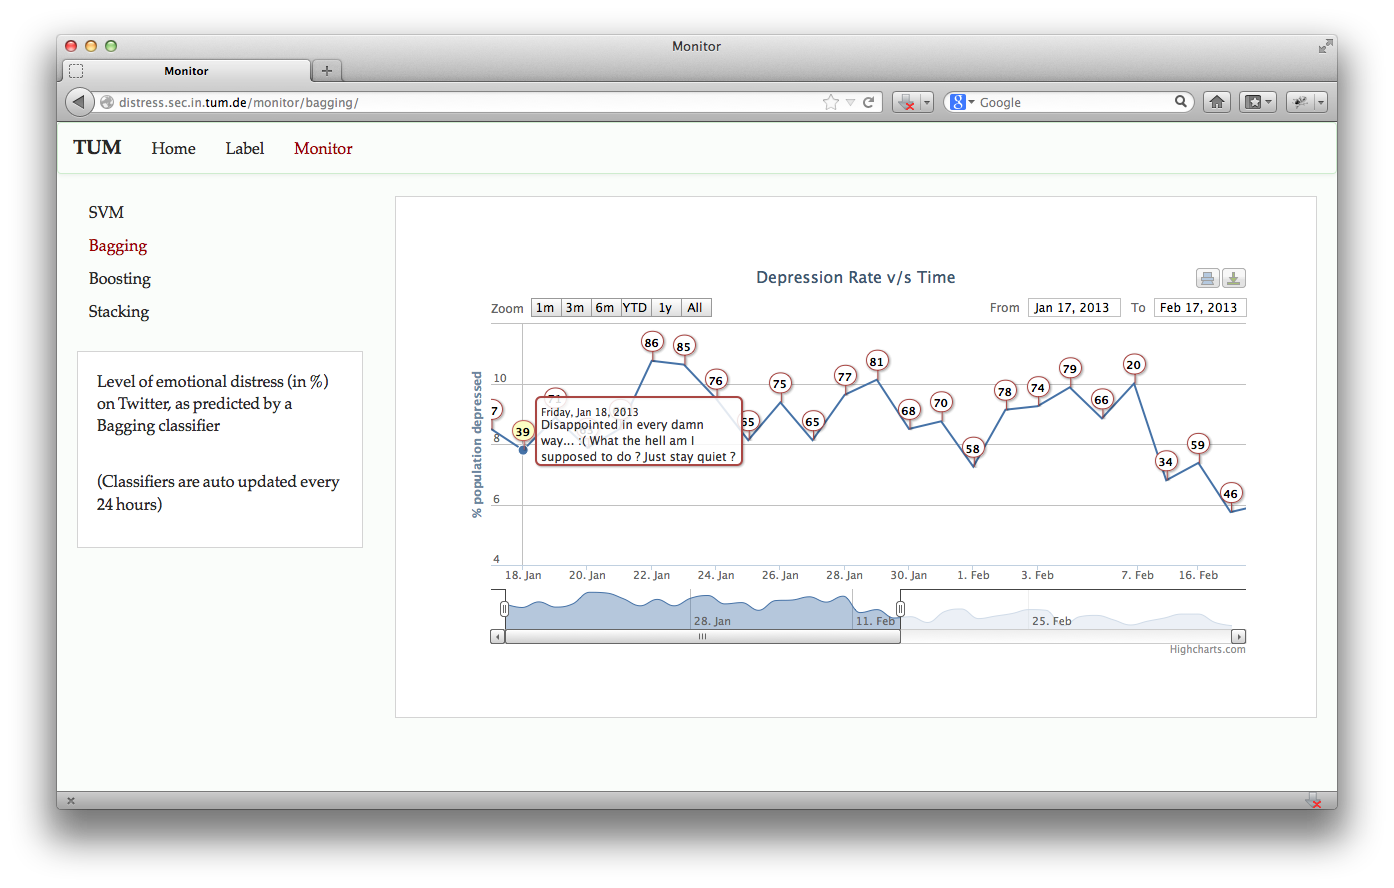
\includegraphics[width=\textwidth]{figures/monitoring_bagging_tweet_info.png}
                    \caption{Statistics of the bagging classifier}
                \end{figure}
            \end{column}
            \begin{column}{0.5\textwidth}
                For each classifier -
                \begin{itemize}
                    \item{displays the overall level of distress (in \%) on Twitter}
                    \item{
                    each bubble displays
                    \begin{itemize}
                        \item{the number of stories that were found depressed on that particular day}
                        \item{the first tweet from that day which was depressed (no confidence values, yet)}
                    \end{itemize}
                    }
                \end{itemize}
            \end{column}
        \end{columns}
    \end{frame}
    
    \begin{frame}
        \begin{center}
            \textbf{Conclusion and Future Work}
        \end{center}
    \end{frame}
    
    \begin{frame}
        \frametitle{Conclusion}
        \begin{itemize}
            \item{An evaluation of Support Vector Machines and Ensemble Learning methods (Bagging/Boosting/Stacking) in the domain of text classification}
            \item{Bagging outperformed Stacking outperformed SVM outperformed Boosting}
            \item{A web based system that can detect emotional distress on Twitter}
            \item{No labels implies qualitative evaluation is difficult except observation}
            \item{Observed results seem to be reasonable}
        \end{itemize}
    \end{frame}
    
    \begin{frame}
        \frametitle{Future Work}
        \begin{itemize}
            \item{Fetch more tweets}
            \item{Increase the crowd intelligence involved}
            \item{Relabelling process (decreases wastage of resources)}
            \item{Select best performing model}
            \item{Store confidence values}
        \end{itemize}
    \end{frame}
    
    \begin{frame}
        \begin{center}
            \textbf{Thank you!}
        \end{center}
        \begin{center}
            \textbf{Questions?}
        \end{center}
    \end{frame}
\end{document}
